\section{Analyse}
L'analyse de l'application se découpe en deux parties. Tout d'abord l'analyse des cas d'utilisation puis les diagrammes de séquence des cas d'utilisation qui méritent à notre sens un éclaircissment sur l'utilisation de l'application.
\subsection{Cas d'utilisation} % (fold)
\label{sub:cas_d_utilisation}
La vision générale des cas d'utilisation est décrite ci-après :
\begin{center}
	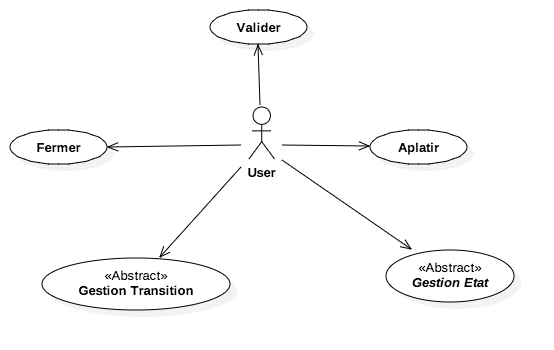
\includegraphics[scale=0.7]{appUC.png}
\end{center}
\newpage
Dans un soucis de clarté nous avons découpé le cas ``Gestion état '' ...
\begin{center}
	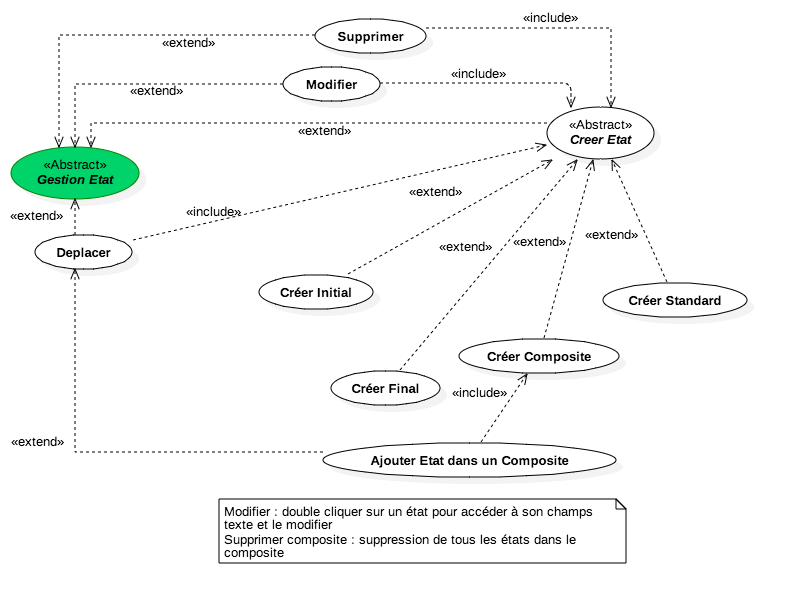
\includegraphics[scale=0.7]{etatUC.png}
\end{center}
\newpage
... et le cas ``Gestion des transtions''
\begin{center}
	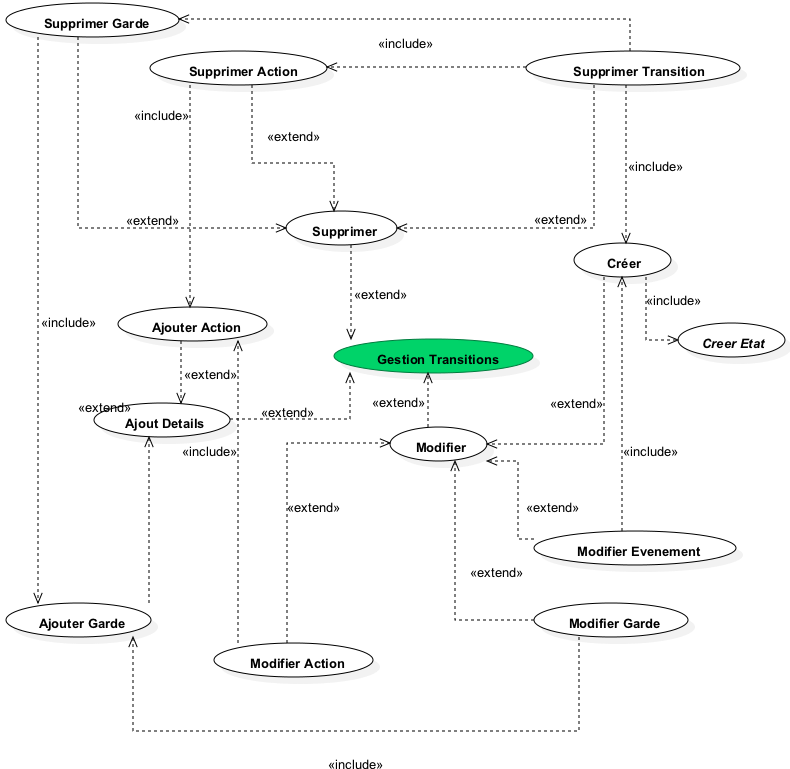
\includegraphics[scale=0.5]{transitionUC.png}
\end{center}
% subsection cas_d_utilisation (end)
\newpage